\documentclass{article}
\title{YOUR PAPER}
\author{ARAVIND}
\usepackage{color}
\usepackage{graphicx}
\date{April-03-24}

\begin{document}
	\maketitle
	\begin{center}
	\textbf{Abstract} 
   \end{center}
	\shortstack{My Abstract}
	\section{Introduction} \label{sec : intro} 
	Your introduction goes here! Simply start writing your document and use the Recompile button to
	view the updated PDF preview. Examples of commonly used commands and features are listed below,
	to help you get started.
	Once you’re familiar with the editor, you can find various project setting in the Overleaf menu,
	accessed via the button in the very top left of the editor. To view tutorials, user guides, and further
	documentation, please visit our \textcolor{blue}{ help library}, or head to our plans page to \textcolor{blue}{choose your plan.}
	\section{Some Examples to Get Started}
	\subsection{How to create Sections and Subsections}
	Simply use the section and subsection commands, as in this example document! With Overleaf, all
	the formatting and numbering is handled automatically according to the template you’ve chosen. If
	you’re using Rich Text mode, you can also create new section and subsections via the buttons in the
	editor toolbar.
	\subsection{How to include Figures}
	First you have to upload the image file from your computer using the upload link in the file-tree menu.
	Then use the includegraphics command to include it in your document. Use the figure environment
	and the caption command to add a number and a caption to your figure. See the code for Figure 1 in
	this section for an example.
	Note that your figure will automatically be placed in the most appropriate place for it, given the
	surrounding text and taking into account other figures or tables that may be close by. You can find
	out more about adding images to your documents in this help article on \textcolor{blue}{including images on Overleaf.}
	\begin{figure}
		\begin{center}
			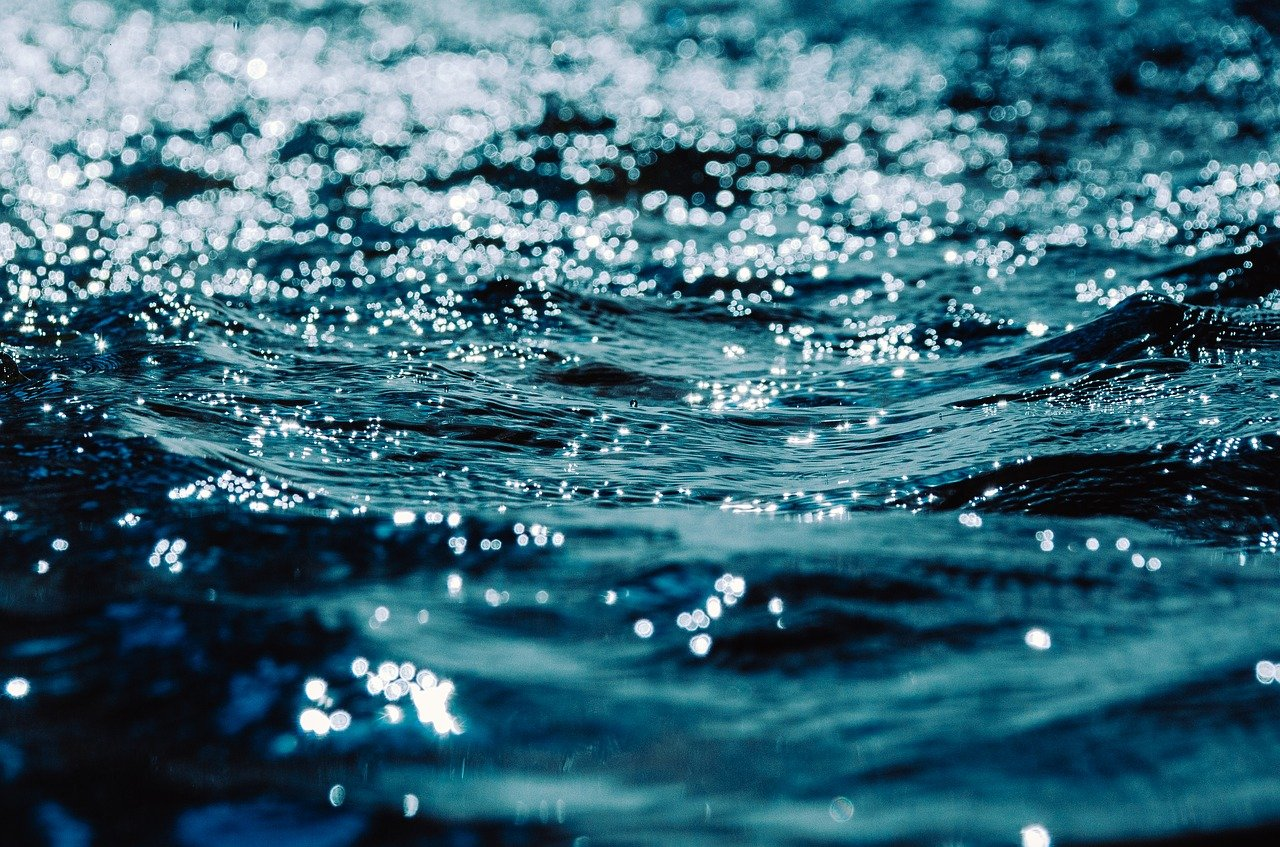
\includegraphics[width=0.6 \linewidth]{img.jpg}
		\end{center}
      \caption{Water}
	\end{figure}

    \begin{table}[h]
    	
   \begin{center}
    \begin{tabular}{|c|c|}
    	\hline
    	  \textbf{item} & 
    	  \textbf{quantity} \\
    	\hline 
    	widgets & 42 \\
    	\hline 
    	gadgets & 13\\
    	\hline
    \end{tabular}
    	\end{center}
        \caption{Example Table}
    \end{table}

  \subsection{How to add Tables}
  Use the table and tabular environments for basic tables — see Table 1, for example. For more infor-
  mation, please see this help article on \textcolor{blue}{tables}
  \subsection{How to add Comments and Track Changes}
\end{document}